\documentclass{../../class}

\title{4231 Homework 6}
\author{Eumin Hong (eh2890)}
\date{\today}

\begin{document}
\maketitle

\lhead{4231 Homework 6}
\rhead{Eumin Hong (eh2890)}

\tcbset{colback=blue!5, colframe=blue!75!black}

\section*{Problem 1}
\begin{tcolorbox}
    Problem 23-4 on Page 641: Alternative minimum-spanning-tree algorithms. For each of the three algorithms, either give a counterexample or prove that it always outputs a minimum spanning tree. Make sure your proof is written clearly and concisely. Also there is no need to describe efficient implementations of these algorithms.
\end{tcolorbox}

\subsection*{23-4}
In this problem, we give pseudocode for three different algorithms. Each on takes a connected graph and a weight function as input and returns a set of edges $T$. For each algorithm, either prove that $T$ is a minimum spanning tree or prove that $T$ is not a minimum spanning tree. Also describe the most efficient implementation of each algorithm, whether or not it computes a minimum spanning tree.
\begin{enumerate}[\textbf{\textit{\alph*.}}]
    \item $\textsc{Maybe-MST-A}(G, w)$
    \begin{algorithmic}[1]
        \State sort the edges into nonincreasing order of edge weights $w$
        \State $T = E$
        \For{each edge $e$, taken in nonincreasing order by weight}
            \If {$T - \{e\}$ is a connected graph}
                \State $T = T - \{e\}$
            \EndIf
        \EndFor\vspace{-0.3em}
        \State \Return $T$
    \end{algorithmic}
    \item $\textsc{Maybe-MST-B}(G, w)$
    \begin{algorithmic}[1]
        \State $T = \emptyset$
        \For{each edge $e$, taken in arbitrary order}
            \If{$T\cup \{e\}$ has no cycles}
                \State $T = T\cup \{e\}$
            \EndIf
        \EndFor\vspace{-0.3em}
        \State \Return $T$
    \end{algorithmic}
    \item $\textsc{Maybe-MST-C}(G, w)$
    \begin{algorithmic}[1]
        \State $T = \emptyset$
        \For{each edge $e$, taken in arbitrary order}
            \State $T = T\cup \{e\}$
            \If {$T$ has a cycle $c$}
                \State let $e'$ be a maximum-weight edge on $c$
                \State $T = T - \{e'\}$
            \EndIf
        \EndFor\vspace{-0.3em}
        \State \Return $T$
    \end{algorithmic}
\end{enumerate}

\newpage
\section*{Problem 2}
\begin{tcolorbox}
    Problem 24-4 on Page 679: Gabow's scaling algorithm for single-source shortest paths.
\end{tcolorbox}

\subsection*{24-4}
\textbf{\textit{Arbitrage}} is the use of discrepancies in currency exchange rates to transform one unit of a currency into more than one unit of the same currency. For example, suppose that $1$ U.S. dollar buys $49$ Indian rupees, $1$ Indian rupee buys $2$ Japanese yen, and $1$ Japanese yen buys $0.0107$ U.S. dollars. Then, by converting currencies, a trader can start with $1$ U.S. dollar and buy $49\times 2 \times 0.0107 = 1.0486$ U.S. dollars, thus turning a profit of $4.86$ percent.

Suppose that we are given $n$ currencies $c_1, c_2, \dots, c_n$ and an $n\times n$ table $R$ of exchange rates, such that one unit of currency $c_i$ buys $R[i, j]$ units of currency $c_j$.

\begin{enumerate}[\textbf{\textit{\alph*.}}]
    \item Give an efficient algorithm to determine whether or not there exists a sequence of currencies $\langle c_{i_1}, c_{i_2}, \dots, c_{i_k} \rangle $ such that
    \begin{gather*}
        R[i_1, i_2]\cdot R[i_2, i_3]\cdots R[i_{k-1}, i_k] \cdot R[i_k, i_1] > 1
    \end{gather*}
    Analyze the running time of your algorithm.
    \item Give an efficient algorithm to print out such a sequence if one exists. Analyze the running time of your algorithm.
\end{enumerate}

\newpage
\section*{Problem 3}
\begin{tcolorbox}
    Problem 25-2 on Page 706: Shortest paths in $\epsilon$-dense graphs. Skip a). For a $d$-ary min-heap, $\textsc{Insert}$ takes time $O(\log_d{n})$; $\textsc{Extract-Min}$ takes time $O(d\cdot \log_d{n})$; and $\textsc{Decrease-Key}$ takes time $O(\log_d{n})$. Check Chapter 6 and Problem 6-2 if you are interested in $d$-ary min-heaps. But for this problem, you may use these facts for free.
\end{tcolorbox}

\subsection*{25-2}
A graph $G = (V, E)$ is $\mathbf{\epsilon}$\textbf{-dense} if $|E| = \Theta(V^{1+\epsilon})$ for some constant $\epsilon$ in the range $0 < \epsilon \leq 1$. By using $d$-ary min-heaps (see Problem 6-2) in shortest-paths algorithms on $\epsilon$-dense graphs, we can match the running times of Fibonacci-heap-based algorithms without using as complicated a data structure.
\begin{enumerate}[\textbf{\textit{\alph*.}}]
    \setcounter{enumi}{1}
    \item Show how to compute shortest paths from a single source on an $\epsilon$-dense directed graph $G = (V, E)$ with no negative-weight edges in $O(E)$ time. (\textit{Hint:} Pick $d$ as a function of $\epsilon$.)
    \item Show how to solve the all-pairs shortest-paths problem on an $\epsilon$-dense directed graph $G = (V, E)$ with no negative-weight edges in $O(VE)$ time.
    \item Show how to solve the all-pairs shortest-paths problem in $O(VE)$ time on an $\epsilon$-dense directed graph $G = (V, E)$ that may have negative-weight edges but has no negative-weight cycles.
\end{enumerate}

\newpage
\section*{Problem 4}
\begin{tcolorbox}
    Problem 26.1 on Page 760: Escape problem.
\end{tcolorbox}

\subsection*{26.1}
An $n\times n$ \textbf{\textit{grid}} is an undirected graph consisting of $n$ rows and $n$ columns of vertices, as shown in Figure \ref{fig:1}. We denote the vertex in the $i$th row and the $j$ th column by $(i, j)$. All vertices in a grid have exactly four neighbors, except fo the boundary vertices, which are the points $(i, j)$ for which $i = 1, i = n, j = 1$, or $j = n$.

Given $m \leq n^2$ starting points $(x_1, y_1), (x_2, y_2), \dots, (x_m, y_m)$ in the grid, the \textbf{\textit{escape problem}} is to determine whether or not there are $m$ vertex-disjoint paths from the starting points to any $m$ different points on the boundary. For example, the grid in Figure \ref{fig:1}(a) has an escape, but the grid in Figure \ref{fig:1}(b) does not.
\begin{figure}[H]
    \centering
    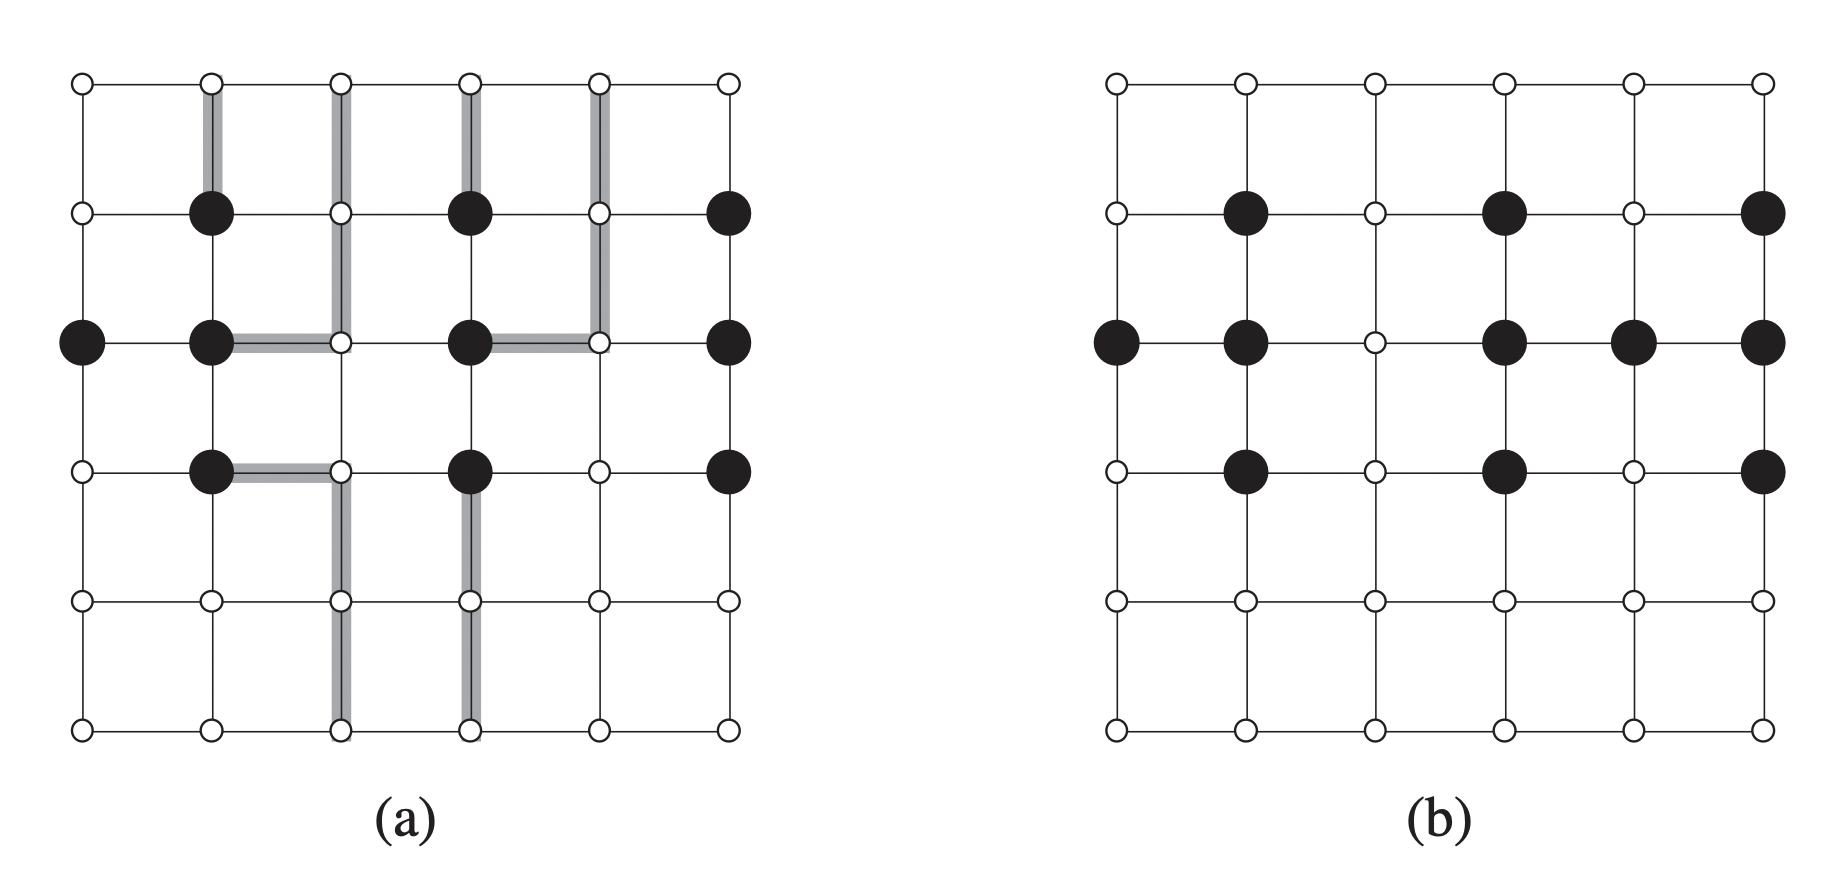
\includegraphics[width = 10cm]{img/1.png}
    \caption{Grids for the escape problem. Starting points are black, and other grid vertices are white. \textbf{(a)} A grid with an escape, shown by shaded paths. \textbf{(b)} A grid with no escape.}
    \label{fig:1}
\end{figure}
\begin{enumerate}[\textbf{\textit{\alph*.}}]
    \item Consider a flow network in which vertices, as well as edges, have capacities. That is, the total positive flow entering any given vertex is subject to a capacity constraint. Show that determining the maximum flow in a network with edge and vertex capacities can be reduced to an ordinary maximum-flow problem on a flow network of comparable size.
    \item Describe an efficient algorithm to solve the escape problem, and analyze its running time.
\end{enumerate}

\end{document}
